\chapter{\linIndepTitle}\label{linearind}

Consider a plane $P$ that includes the origin in $\Re^3$ and non-zero vectors $\{u,v,w\}$ in $P$.
\begin{center}
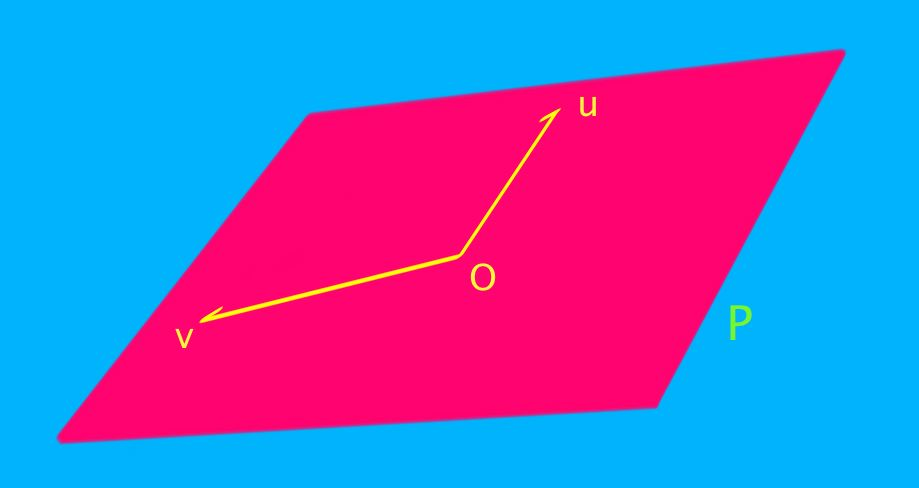
\includegraphics[scale=.3]{\linIndepPath/span_plane.jpg}
\end{center}
If no two of $u, v$ and $w$ are parallel, then $P=\spa \{u,v,w\}$.  But any two vectors determines a plane, so we should be able to span the plane using only two of the vectors $u,v,w$.  Then we could choose two of the vectors in $\{u,v,w\}$ whose span is $P$, and express the other as a linear combination of those two.  Suppose $u$ and $v$ span $P$.  Then there exist constants $d^1, d^2$ (not both zero) such that
$w=d^1u+d^2v$.  Since $w$ can be expressed in terms of $u$ and $v$ we say that it is not independent.
More generally, the relationship
\[
c^1u+c^2v+c^3w=0 \qquad c^i \in \Re, \text{ some $c^i\neq 0$}
\]
expresses the fact that $u,v,w$ are not all independent.

\begin{definition}
\label{independent}
We say that the vectors $v_1, v_2, \ldots, v_n$ are {\bfseries linearly dependent}\index{Linearly dependent} if there exist constants\footnote{Usually our vector spaces are defined over \(\mathbb{R}\), but in general we can have vector spaces defined over different base fields such as \(\mathbb{C}\) or \(\mathbb{Z}_2\). The coefficients \(c^i\) should come from whatever our base field is (usually \(\mathbb{R}\)).} $c^1, c^2, \ldots, c^n$ not all zero such that
\[
c^1v_1 + c^2v_2+ \cdots +c^nv_n=0.
\]
Otherwise, the vectors $v_1, v_2, \ldots, v_n$ are {\bfseries linearly independent.}\index{Linearly independent} 
\end{definition}

\begin{remark}
The zero vector $0_V$ can {\itshape never} be on a list of independent vectors because $\alpha 0_V=0_V$ for any scalar $\alpha$.
\end{remark}

\begin{example}
Consider the following vectors in \(\Re^3\):
\[
v_1=\colvec{4\\-1\\3}, \qquad
v_2=\colvec{-3\\7\\4}, \qquad
v_3=\colvec{5\\12\\17}, \qquad
v_4=\colvec{-1\\1\\0}.
\]
Are these vectors linearly independent?

No, since \(3v_1+2v_2-v_3+v_4=0\), the vectors are linearly {\itshape dependent}.
\end{example}

\Videoscriptlink{linear_independence_example.mp4}{Worked Example}{linear_independence_example}

\section{Showing Linear Dependence}
In the above example we were given the linear combination \(3v_1+2v_2-v_3+v_4\) seemingly by magic. The next example shows how to find such a linear combination, if it exists.

\begin{example}
Consider the following vectors in $\Re^3$:
\[
v_1=\colvec{0\\0\\1}, 
\qquad v_2=\colvec{1\\2\\1},
\qquad v_3=\colvec{1\\2\\3}.
\]
Are they linearly independent?

We need to see whether the system 
\[
c^1v_1 + c^2v_2+ c^3v_3=0
\]
has any solutions for $c^1, c^2, c^3$.  We can rewrite this as a homogeneous system by building a matrix whose columns are the vectors $v_1$, $v_2$ and $v_3$:
\[
\rowvec{v_1&v_2&v_3}\colvec{c^1\\c^2\\c^3}=0.
\]
This system has solutions if and only if the matrix $M=\rowvec{v_1&v_2&v_3}$ is singular, so we should find the determinant of $M$:
\[
\det M = \det \begin{pmatrix}
0 & 1 & 1 \\
0 & 2 & 2 \\
1 & 1 & 3 \\
\end{pmatrix}
= \det \begin{pmatrix}
1 & 1 \\
2 & 2 \\
\end{pmatrix}
=0.
\]

Therefore nontrivial solutions exist.  At this point we know that the vectors are linearly dependent.  If we need to, we can find coefficients that demonstrate linear dependence by solving
\[
\begin{amatrix}{3}
0 & 1 & 1 & 0\\
0 & 2 & 2 & 0\\
1 & 1 & 3 & 0\\
\end{amatrix} \sim
\begin{amatrix}{3}
1 & 1 & 3 & 0\\
0 & 1 & 1 & 0\\
0 & 0 & 0 & 0\\
\end{amatrix} \sim
\begin{amatrix}{3}
1 & 0 & 2 & 0\\
0 & 1 & 1 & 0\\
0 & 0 & 0 & 0\\
\end{amatrix}.
\]
The solution set  $\{ \mu ( -2,-1,1) ~| ~\mu \in \mathbb{R} \}$ encodes the linear combinations equal to zero;  any choice of $\mu$ will produce coefficients $c^1,c^2,c^3$ that satisfy the linear homogeneous equation.  
In particular, $\mu=1$ corresponds to the equation
\[
c^1v_1 + c^2v_2+ c^3v_3=0 
\Rightarrow -2v_1 - v_2 + v_3=0.
\]
\end{example}

\Reading{LinearIndependence}{1}
%\begin{center}\href{\webworkurl ReadingHomework16/1/}{Reading homework: problem \ref{linearind}.1}\end{center}

\begin{definition}
Any sum of vectors $v_1,\ldots, v_k$ multiplied by scalars $c^1,\ldots,c^k$, namely
\[
c^1 v_1+\cdots + c^k v_k\, ,
\]
is called a {\itshape linear combination}\index{Linear combination} of $v_1,\ldots , v_k$.
\end{definition}

\begin{theorem}[Linear Dependence]\index{Linear dependence theorem}
\label{linear_dependence}
An ordered set of non-zero vectors $( v_1, \ldots, v_n )$ is linearly dependent if and only if one of the vectors $v_k$ is expressible as a linear combination of the preceding vectors.
\end{theorem}

\begin{proof}
The theorem is an if and only if statement, so there are two things to show.

\begin{itemize}
\item[$i.$]  First, we show that if $v_k=c^1v_1+\cdots c^{k-1}v_{k-1}$ then the set is linearly dependent.

This is easy.  We just rewrite the assumption:
\[
c^1v_1+\cdots+c^{k-1}v_{k-1}-v_k + 0v_{k+1}+\cdots +0v_n=0.
\]
This is a vanishing linear combination of the vectors $\{ v_1, \ldots, v_n \}$ with not all coefficients equal to zero, so $\{ v_1, \ldots, v_n \}$ is a linearly dependent set.
 
\item[$ii.$]  Now we show that linear dependence implies that there exists $k$ for which $v_k$ is a linear combination of the vectors $\{ v_1, \ldots, v_{k-1} \}$.

The assumption says that
\[
c^1v_1 + c^2v_2+ \cdots +c^nv_n=0.
\]
Take $k$ to be the largest number for which $c_k$ is not equal to zero.  So:
\[
c^1v_1 + c^2v_2+ \cdots +c^{k-1}v_{k-1}+c^kv_k=0.
\]

(Note that $k>1$, since otherwise we would have $c^1v_1=0\Rightarrow v_1=0$, contradicting the assumption that none of the $v_i$ are the zero vector.)

So we can rearrange the equation:
\begin{align*}
c^1v_1 + c^2v_2+ \cdots +c^{k-1}v_{k-1}&=-c^kv_k\\
\Rightarrow\ 
-\frac{c^1}{c^k}v_1 - \frac{c^2}{c^k}v_2 - \cdots -\frac{c^{k-1}}{c^k}v_{k-1}&=v_k.
\end{align*}

Therefore we have expressed $v_k$ as a linear combination of the previous vectors, and we are done.
\end{itemize}
\end{proof}

\Videoscriptlink{linear_independence_thm.mp4}{Worked proof}{scripts_linear_independence_thm}

\begin{example}
Consider the vector space $P_2(t)$ of polynomials of degree less than or equal to $2$.  Set:
\begin{align*}
v_1 &= 1+t \\
v_2 &= 1+t^2 \\
v_3 &= t+t^2 \\
v_4 &= 2+t+t^2 \\
v_5 &= 1+t+t^2. \\
\end{align*}
The set $\{ v_1, \ldots, v_5 \}$ is linearly dependent, because $v_4 = v_1+v_2$.  
\end{example}

\section{Showing Linear Independence} 
We have seen two different ways to show a set of vectors is linearly dependent: we can either find a linear combination of the vectors which is equal to zero, or we can express one of the vectors as a linear combination of the other vectors. On the other hand, to check that a set of vectors is linearly {\itshape independent}, we must check that every  linear combination of our vectors with non-vanishing coefficients gives something other than the zero vector. Equivalently, to show that the set \(v_1, v_2, \ldots, v_n\) is linearly independent, we must show that the equation \(c_1 v_1+c_2v_2 + \cdots + c_n v_n=0\) has no solutions other than \(c_1=c_2=\cdots=c_n=0.\)

\begin{example}
Consider the following vectors in $\Re^3$:
\[
v_1=\colvec{0\\0\\2},
\qquad v_2=\colvec{2\\2\\1},
\qquad v_3=\colvec{1\\4\\3}.
\]
Are they linearly independent?

We need to see whether the system
\[
c^1v_1 + c^2v_2+ c^3v_3=0
\]
has any solutions for $c^1, c^2, c^3$.  We can rewrite this as a homogeneous system:
\[
\rowvec{v_1&v_2&v_3}\colvec{c^1\\c^2\\c^3}=0.
\]
This system has solutions if and only if the matrix $M=\rowvec{v_1&v_2&v_3}$ is singular, so we should find the determinant of $M$:
\[
\det M = \det \begin{pmatrix}
0 & 2 & 1 \\
0 & 2 & 4 \\
2 & 1 & 3 \\
\end{pmatrix}
= 2 \det \begin{pmatrix}
2 & 1 \\
2 & 4 \\
\end{pmatrix}
=12.
\]
Since the matrix \(M\) has non-zero determinant, the only solution to the system of equations
\[
\rowvec{v_1&v_2&v_3}\colvec{c^1\\c^2\\c^3}=0
\]
is \(c_1=c_2=c_3=0\). So the vectors \(v_1, v_2, v_3\) are linearly independent.
\end{example}

Here is another example with bits:

\begin{example}
Let $\mathbb{Z}_2^3$ be the space of $3\times 1$ bit-valued matrices (i.e., column vectors).  Is the following subset linearly independent?
\[
\left\{ \colvec{1\\1\\0}, \colvec{1\\0\\1}, 
\colvec{0\\1\\1} \right\}
\]

If the set is linearly dependent, then we can find non-zero solutions to the system:
\[
c^1\colvec{1\\1\\0}+ c^2 \colvec{1\\0\\1} 
+c^3 \colvec{0\\1\\1}=0,
\]
which becomes the linear system
\[
\begin{pmatrix}
1 & 1 & 0 \\
1 & 0 & 1 \\
0 & 1 & 1 \\
\end{pmatrix}\colvec{c^1\\c^2\\c^3}=0.
\]
Solutions exist if and only if the determinant of the matrix is non-zero.  But:
\[
\det \begin{pmatrix}
1 & 1 & 0 \\
1 & 0 & 1 \\
0 & 1 & 1 \\
\end{pmatrix} = 1 \det \begin{pmatrix}
0 & 1 \\
1 & 1 \\
\end{pmatrix} -1 \det \begin{pmatrix}
1 & 1 \\
0 & 1 \\
\end{pmatrix} = -1-1=1+1=0
\]
Therefore non-trivial solutions exist, and the set is not linearly independent.

\end{example}


\Reading{LinearIndependence}{2}
%\begin{center}\href{\webworkurl ReadingHomework16/2/}{Reading homework: problem \ref{linearind}.2}\end{center}

\section{From Dependent Independent } 
Now suppose vectors 
$v_1,\ldots, v_n$ are linearly dependent, 
\[
c^1v_1 + c^2v_2+ \cdots +c^nv_n=0
\]
with $c^1\neq 0$.  Then:
\[
\spa \{v_1,\ldots, v_n\} = \spa \{ v_2,\ldots, v_n\}
\]
because any $x\in \spa \{v_1,\ldots, v_n\}$ is given by
\begin{align*}
x &= a^1v_1 + \cdots+ a^nv_n \\
&= a^1\left( -\frac{c^2}{c_1}v_2- \cdots -\frac{c^n}{c_1}v_n \right) + a^2v_2 + \cdots + a^nv_n \\
&= \left(a^2-a^1\frac{c^2}{c_1}\right)v_2 + \cdots + \left(a^n-a^1\frac{c^n}{c_1}\right)v_n.
\end{align*}
Then $x$ is in $\spa \{v_2,\ldots, v_n\}$.

When we write a vector space as the span of a list of vectors, we would like that list to be as short as possible (this idea is explored further in \hyperref[dimension]{chapter~\ref*{sec:dimension}}).
This can be achieved by iterating the above procedure.

\begin{example}
In the above example, we found that $v_4=v_1+v_2$.  In this case, any expression for a vector as a linear combination involving $v_4$ can be turned into a combination without $v_4$ by making the substitution $v_4=v_1+v_2$.

Then:
\begin{align*}
S &= \spa \{ 1+t , 1+t^2, t+t^2, 2+t+t^2, 1+t+t^2 \} \\
&= \spa \{ 1+t , 1+t^2, t+t^2, 1+t+t^2 \}.
\end{align*}
Now we notice that $1+t+t^2=\frac{1}{2}(1+t) +\frac{1}{2}(1+t^2) + \frac{1}{2}(t+t^2)$.  So the vector $1+t+t^2=v_5$ is also extraneous, since it can be expressed as a linear combination of the remaining three vectors, $v_1, v_2,v_3$.  Therefore 
\[
S = \spa \{ 1+t , 1+t^2, t+t^2 \}.
\]

In fact, you can check that there are no (non-zero) solutions to the linear system
\[
c^1(1+t) + c^2(1+t^2) + c^3(t+t^2)=0.
\]
Therefore the remaining vectors $\{ 1+t , 1+t^2, t+t^2 \}$ are linearly independent, and span the vector space $S$.  Then these vectors are a minimal spanning set\index{Minimal spanning set}, in the sense that no more vectors can be removed since the vectors are linearly independent.
Such a set is called a \emph{basis}\index{Basis!example of} for $S$.
\end{example}





%To summarize, the key definition in this lecture was:
%\begin{center}
%
\includegraphics[scale=.3]{\linIndepPath/linear_dependent.jpg}
%\end{center}
%Perhaps the most useful Theorem was:
%\begin{center}
%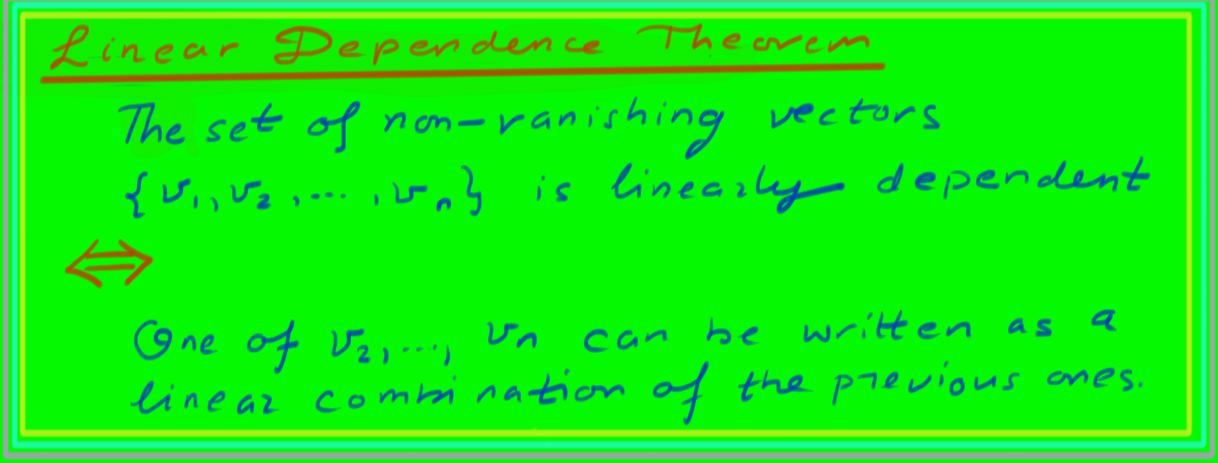
\includegraphics[scale=.3]{\linIndepPath/linear_dependence_thm.jpg}
%\end{center}

%\section*{References}
%Hefferon, Chapter Two, Section II: Linear Independence
%\\
%Hefferon, Chapter Two, Section III.1: Basis
%\\
%Beezer, Chapter V, Section LI
%\\
%Beezer, Chapter V, Section LDS
%\\
%Beezer, Chapter VS, Section LISS, Subsection LI
%\\
%Wikipedia:
%\begin{itemize}
%\item \href{http://en.wikipedia.org/wiki/Linear_independence}{Linear Independence}
%\item \href{http://en.wikipedia.org/wiki/Basis_(linear_algebra)}{Basis}
%\end{itemize}

\section{Review Problems}
{\bfseries Webwork:} 
\begin{tabular}{|c|c|}
\hline
Reading Problems & 
 \hwrref{LinearIndependence}{1},\hwrref{LinearIndependence}{2}\\
 Testing for linear independence &\hwref{LinearIndependence}{3},
 \hwref{LinearIndependence}{4}\\
 Gaussian elimination &\hwref{LinearIndependence}{5}\\
 Spanning and linear independence &\hwref{LinearIndependence}{6}\\
  \hline
\end{tabular}





\begin{enumerate}
\item \label{det33} Let $M=\begin{pmatrix}
m^1_1 & m^1_2 & m^1_3\\
m^2_1 & m^2_2 & m^2_3\\
m^3_1 & m^3_2 & m^3_3\\
\end{pmatrix}$.  Use row operations to put $M$ into \emph{row echelon form}.  For simplicity, assume that $m_1^1\neq 0 \neq m^1_1m^2_2-m^2_1m^1_2$.

Prove that $M$ is non-singular if and only if:
\[
m^1_1m^2_2m^3_3 
- m^1_1m^2_3m^3_2 
+ m^1_2m^2_3m^3_1 
- m^1_2m^2_1m^3_3 
+ m^1_3m^2_1m^3_2
- m^1_3m^2_2m^3_1
\neq 0
\]

\phantomnewpage

\item 
\begin{enumerate}
\item What does the matrix $E^1_2=\begin{pmatrix}
0 & 1 \\
1 & 0
\end{pmatrix}$ do to $M=\begin{pmatrix}
a & b \\
d & c
\end{pmatrix}$ under left multiplication?  What about right multiplication?
\item Find elementary matrices $R^1(\lambda)$ and $R^2(\lambda)$ that respectively multiply rows $1$ and $2$ of $M$ by $\lambda$ but otherwise leave $M$ the same under left multiplication.
\item Find a matrix $S^1_2(\lambda)$ that adds a multiple $\lambda$ of row $2$ to row $1$ under left multiplication.
\end{enumerate}

\phantomnewpage

\item Let $M$ be a matrix and $S^i_jM$ the same matrix with rows \(i\) and \(j\) switched.  Explain every line of the 
\hyperlink{rowswap}{series of equations} proving that $\det M = -\det (S^i_jM)$.

\phantomnewpage

%\item \label{prob_inversion_number} This problem is a ``hands-on'' look at why \hyperlink{permutation_parity}{the property} describing the parity of permutations is true.
%
%\hypertarget{inversion_number}{The \emph{inversion number}}\index{Permutation!Inversion number} of a permutation $\sigma$ is the number of pairs $i<j$ such that $\sigma(i)>\sigma(j)$; it's the number of ``numbers that appear left of smaller numbers'' in the permutation.  For example, for the permutation $\rho = [4,2,3,1]$, the inversion number is $5$. The number $4$ comes before $2,3,$ and $1$, and $2$ and $3$ both come before $1$.
%
%Given a permutation $\sigma$, we can make a new permutation $\tau_{i,j} \sigma$ by exchanging the $i$th and $j$th entries of $\sigma$.
%
%\begin{enumerate}
%\item What is the inversion number of the permutation \(\mu=[1,2,4,3]\) that exchanges 4 and 3 and leaves everything else alone? Is it an even or an odd permutation?
%
%\item What is the inversion number of the permutation \(\rho=[4,2,3,1]\) that exchanges 1 and 4 and leaves everything else alone? Is it an even or an odd permutation?
%
%\item What is the inversion number of the permutation \(\tau_{1,3} \mu\)? Compare the parity\footnote{The \emph{parity} of an integer refers to whether the integer is even or odd. Here the parity of a permutation $\mu$ refers to the parity of its inversion number.} of \(\mu\) to the parity of \(\tau_{1,3} \mu.\)
%
%\item What is the inversion number of the permutation \(\tau_{2,4} \rho\)? Compare the parity of \(\rho\) to the parity of \(\tau_{2,4} \rho.\)
%
%\item What is the inversion number of the permutation \(\tau_{3,4} \rho\)? Compare the parity of \(\rho\) to the parity of \(\tau_{3,4} \rho.\)
%\end{enumerate}
%
%\videoscriptlink{elementary_matrices_determinant_hint.mp4}{Problem~\ref{prob_inversion_number} hints}{scripts_elementary_matrices_determinants_hint}

\phantomnewpage

%\item \label{problem_permutation} (Extra credit) Here we will examine a (very) small set of the general properties about permutations and their applications. In particular, we will show that one way to compute the sign of a permutation is by finding the \hyperlink{inversion_number}{inversion number} $N$ of $\sigma$ and we have
%\[
%\sgn(\sigma) = (-1)^N.
%\]
%
%For this problem, let $\mu = [1,2,4,3]$.
%
%\begin{enumerate}
%\item Show that every permutation $\sigma$ can be sorted by only taking simple (adjacent) transpositions\index{Permutation!Simple transposition} $s_i$ where $s_i$ interchanges the numbers in position $i$ and $i+1$ of a permutation $\sigma$ (in our other notation $s_i = \tau_{i,i+1}$). For example $s_2 \mu = [1, 4, 2, 3]$, and to sort $\mu$ we have $s_3 \mu = [1, 2, 3, 4]$.
%
%\item \label{prob_part_relations} We can compose simple transpositions together to represent a permutation (note that the sequence of compositions is not unique), and these are associative, we have an identity (the trivial permutation where the list is in order or we do nothing on our list), and we have an inverse since it is clear that $s_i s_i \sigma = \sigma$. Thus permutations of $[n]$ under composition are an example of a \hyperref[groups]{group}. However note that not all simple transpositions commute with each other since
%\begin{align*}
%s_1 s_2 [1, 2, 3] & = s_1 [1, 3, 2] = [3, 1, 2]
%\\ s_2 s_1 [1, 2, 3] & = s_2 [2, 1, 3] = [2, 3, 1]
%\end{align*}
%(you will prove here when simple transpositions commute). When we consider our initial permutation to be the trivial permutation $e = [1, 2, \dotsc, n]$, we do not write it; for example $s_i \equiv s_i e$ and $\mu = s_3 \equiv s_3 e$. This is analogous to not writing 1 when multiplying. Show that $s_i s_i = e$ (in shorthand $s_i^2 = e$), $s_{i+1} s_i s_{i+1} = s_i s_{i+1} s_i$ for all $i$, and $s_i$ and $s_j$ commute for all $|i - j| \geq 2$.
%
%\item Show that every way of expressing $\sigma$ can be obtained from using the relations proved in part~\ref{prob_part_relations}. In other words, show that for any expression $w$ of simple transpositions representing the trivial permutation $e$, using the proved relations.
%
%\emph{Hint: Use induction on $n$. For the induction step, follow the path of the $(n+1)$-th strand by looking at $s_n s_{n-1} \cdots s_k s_{k\pm1} \cdots s_n$ and argue why you can write this as a subexpression for any expression of $e$. Consider using diagrams of these paths to help.}
%
%\item The simple transpositions \hyperlink{action}{acts on} an $n$-dimensional vector space $V$ by $s_i v = E^i_{i+1} v$ (where $E^i_j$ is \hyperlink{elem_matrix_row_swap}{an elementary matrix}) for all vectors $v \in V$. Therefore we can just represent a permutation $\sigma$ as the matrix $M_{\sigma}$\footnote{Often people will just use $\sigma$ for the matrix when the context is clear.}, and we have $\det(M_{s_i}) = \det(E^i_{i+1}) = -1$. Thus prove that $\det(M_{\sigma}) = (-1)^N$ where $N$ is a number of simple transpositions needed to represent $\sigma$ as a permutation. You can assume that $M_{s_i s_j} = M_{s_i} M_{s_j}$ (it is not hard to prove) and that $\det(A B) = \det(A) \det(B)$ \hyperref[detmultiplicative]{from Chapter~\ref*{elementarydeterminantsII}}.
%
%\emph{Hint: You to make sure $\det(M_{\sigma})$ is well-defined since there are infinite ways to represent $\sigma$ as simple transpositions.}
%
%\item Show that $s_{i+1} s_i s_{i+1} = \tau_{i, i+2}$, and so give one way of writing $\tau_{i, j}$ in terms of simple transpositions? Is $\tau_{i,j}$ an even or an odd permutation? What is $\det(M_{\tau_{i,j}})$? What is the inversion number of $\tau_{i,j}$?
%
%\item The minimal number of simple transpositions needed to express $\sigma$ is called the \emph{length}\index{Permutation!Length} of $\sigma$; for example the length of $\mu$ is 1 since $\mu = s_3$. Show that the length of $\sigma$ is equal to the inversion number of $\sigma$.
%
%\emph{Hint: Find an procedure which gives you a new permutation $\sigma^{\prime}$ where $\sigma = s_i \sigma^{\prime}$ for some $i$ and the inversion number for $\sigma^{\prime}$ is 1 less than the inversion number for $\sigma$.}
%
%\item Show that $(-1)^N = \sgn(\sigma) = \det(M_{\sigma})$, where $\sigma$ is a permutation with $N$ inversions. Note that this immediately implies that $\sgn(\sigma \rho) = \sgn(\sigma) \sgn(\rho)$ for any permutations $\sigma$ and $\rho$.
%\end{enumerate}

\item Let $M'$ be the matrix obtained from $M$ by swapping two columns $i$ and $j$. Show that $\det M'=-\det M $.

\item The scalar triple product of three vectors $u,v,w$ from $\Re^3$ is $u\cdot(v\times w)$. Show that this product is the same as the determinant of the matrix whose columns are $u,v,w$ (in that order). What happens to the scalar triple product when the factors are permuted? 

\item Show that if $M$ is a $3\times 3$ matrix whose third row is a sum of multiples of the other rows ($R_3=aR_2+bR_1$) then $\det M=0$. Show that the same is true if one of the columns is a sum of multiples of the others. 

\end{enumerate}

\phantomnewpage


